\subsection{Настройка внешнего вида системы}

\subparagraph{1) Что нужно было сделать?}

Настройте под себя внешний вид системы, опишите весь процесс настройки в отчете.

\subparagraph{2) Как это сделали?}

В меню есть кнопка <<Settings Managment>>.
Рисунок~\ref{fig:Settings-Managment}
(стр.~\pageref{fig:Settings-Managment}).

В Keyboard - можно добавить язык и настроить кнопки переключения языка.
Рисунок~\ref{fig:Keyboard}
(стр.~\pageref{fig:Keyboard}).

В Windows Manager - можно добавить кнопки там, где заголовок программы, и выбрать тему окна.
Рисунок~\ref{fig:Window-Manager}
(стр.~\pageref{fig:Window-Manager}).

В Panel - можно создать панели и добавить туда элементов.
Рисунок~\ref{fig:Panel}
(стр.~\pageref{fig:Panel}).

В Appearance - можно настроить иконки.
Рисуноки~\ref{fig:Apperance-icons}~и~\ref{fig:Apperance-style}
(стр.~\pageref{fig:Apperance-icons}~и~\pageref{fig:Apperance-style}).

\begin{figure}[!htp]
    \begin{minipage}{0.49\textwidth}
        \centering
        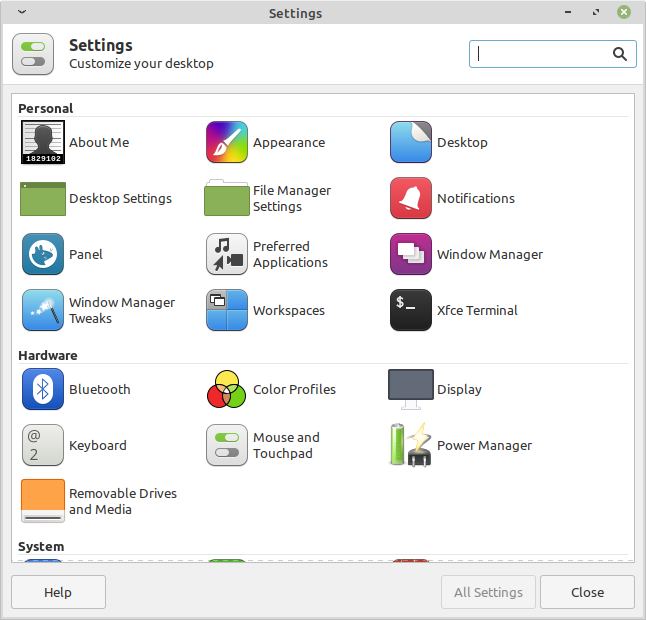
\includegraphics[width=\linewidth]
            {../input/task-2/3/Settings-Managment.png}
        \caption{Settings-Managment}
        \label{fig:Settings-Managment}
    \end{minipage}
    \begin{minipage}{0.49\textwidth}
        \centering
        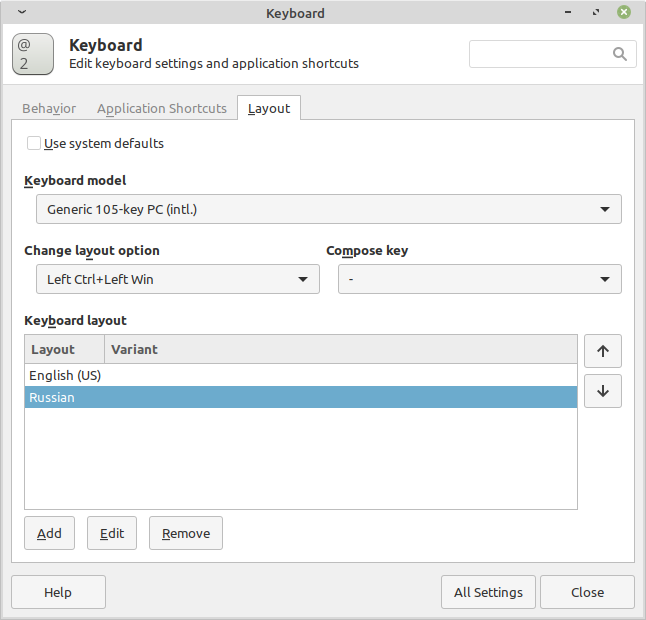
\includegraphics[width=\linewidth]
            {../input/task-2/3/Keyboard.png}
        \caption{Keyboard}
        \label{fig:Keyboard}
    \end{minipage}
\end{figure}

\begin{figure}[!htp]
    \begin{minipage}{0.49\textwidth}
        \centering
        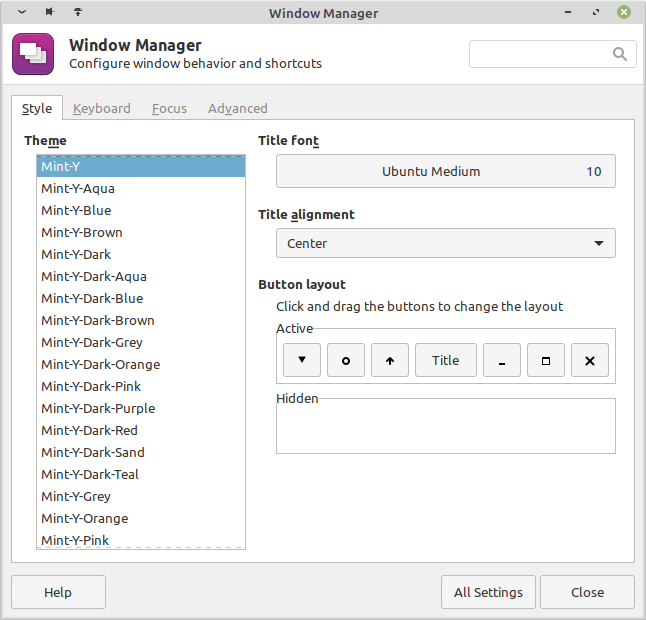
\includegraphics[width=\linewidth]
            {../input/task-2/3/Window-Manager.png}
        \caption{Window-Manager}
        \label{fig:Window-Manager}
    \end{minipage}
    \begin{minipage}{0.49\textwidth}
        \centering
        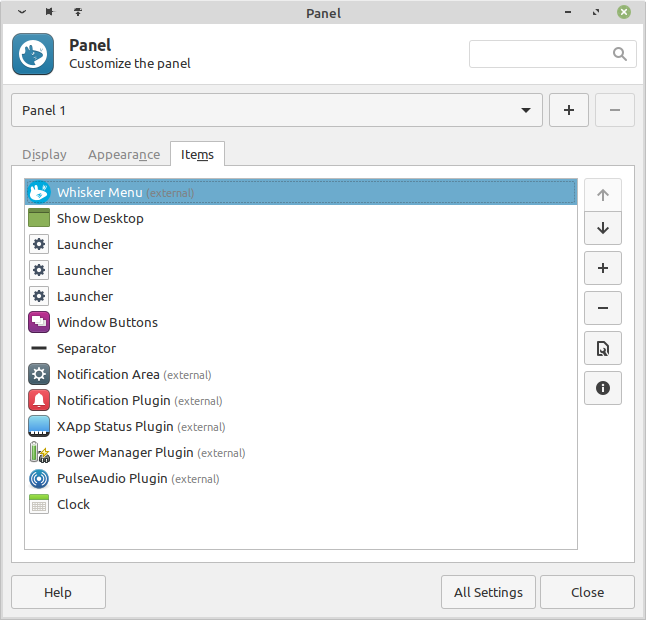
\includegraphics[width=\linewidth]
            {../input/task-2/3/Panel.png}
        \caption{Panel}
        \label{fig:Panel}
    \end{minipage}
\end{figure}

\begin{figure}[!htp]
    \begin{minipage}{0.49\textwidth}
        \centering
        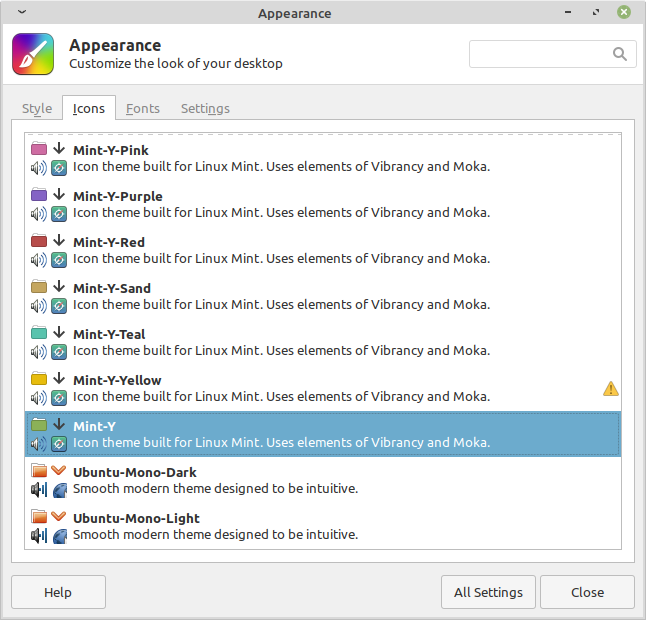
\includegraphics[width=\linewidth]
            {../input/task-2/3/Apperance-icons.png}
        \caption{Apperance-icons}
        \label{fig:Apperance-icons}
    \end{minipage}
    \begin{minipage}{0.49\textwidth}
        \centering
        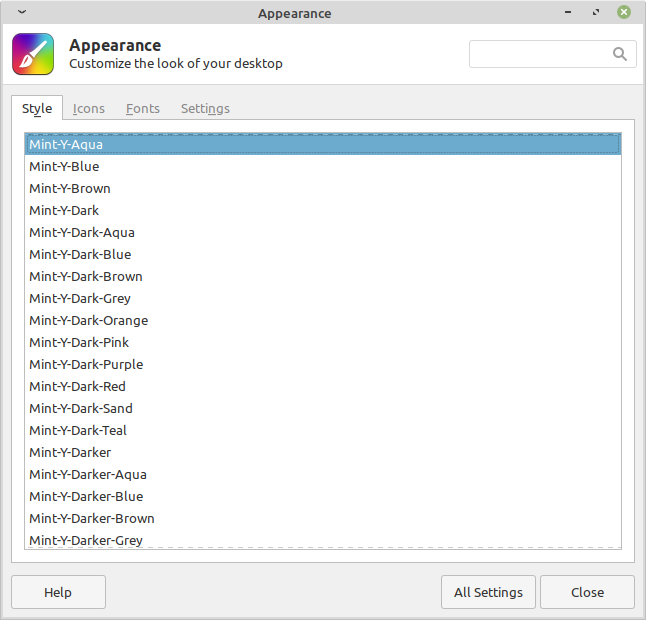
\includegraphics[width=\linewidth]
            {../input/task-2/3/Apperance-style.png}
        \caption{Apperance-style}
        \label{fig:Apperance-style}
    \end{minipage}
\end{figure}

\subparagraph{3) Что получилось?}

Открыли утилиту Synaptic. Через поиск проверили установленность пакетов.
